\documentclass[a4paper,12pt]{report}

\usepackage{alltt, fancyvrb, url}
\usepackage{graphicx}
\usepackage[utf8]{inputenc}
\usepackage{float}
\usepackage{xcolor}
\usepackage{hyperref}

\usepackage[italian]{babel}

\usepackage[italian]{cleveref}
\title{Relazione di Progetto \\ Web Server e Sito Web}
\author{Giovanni Maria Rava}
\date{\today}
\begin{document}
\maketitle
\tableofcontents
\chapter{Introduzione}
Questa relazione documenta lo sviluppo di un semplice Web Server scritto in linguaggio Python (versione 3.12), in grado di gestire 
richieste HTTP e servire contenuti statici in formato HTML e CSS. Il progetto ha finalità didattiche ed è stato realizzato nell’ambito
del corso di Programmazione di Reti (codice: 70226), durante l’Anno Accademico 2024/2025.

Durante lo sviluppo del progetto sono stati utilizzati diversi ambienti di lavoro e strumenti di sviluppo, elencati di seguito:
\begin{itemize}
    \item \textbf{Spyder 6}, per il debugging interattivo del codice Python;
    \item \textbf{Visual Studio Code}, per l’editing del codice e la gestione dei file HTML/CSS;
    \item \textbf{GitHub}, per il versionamento e l’archiviazione del progetto.
\end{itemize}
\section{Obbiettivo}
Progettare un semplice server HTTP in Python (usando socket) e servire un sito web statico con HTML/CSS.
\section{Requisiti minimi}
\begin{itemize}
    \item Il server deve rispondere su localhost:8080
    \item Deve servire almeno tre pagine HTML statiche
    \item Gestione di richieste GET e risposta con codice 200
    \item Implementare risposta 404 per file inesistenti 
\end{itemize}
\section{Estensioni opzionali}
\begin{itemize}
    \item Gestione dei MIME types (.html, .css, .jpg)
    \item Logging delle richieste
    \item Aggiunta di animazioni o layout responsive
\end{itemize}
\chapter{Fondamenti Teorici}
\section{Protocollo HTTP}
Il Hypertext Transfer Protocol (HTTP) è il protocollo standard per la comunicazione tra client e server sul Web . HTTP funziona secondo
un modello stateless, ovvero ogni transazione è indipendente e non si tiene memoria di essa. Utilizza comandi testuali standard come 
GET per richiedere risorse. All'interno di HTTP sono prensenti messaggi di due tipi:
\begin{itemize}
    \item richiesta
    \item risposta
\end{itemize}
Ogni messaggio è formato da una intestazione (\emph{header}) seguita dal corpo (\emph{body}). L'intestazione è composta da una serie di righe di testo
terminate da caratteri di fine linea. Una richiesta inizia con una riga di richiesta, seguita da una o più righe di intestazione. Una 
risposta inizia con una riga di stato, seguita da una o più righe di intestazione. All'interno del body vengono contenuti i dati da 
trasferire. 

In questo progetto viene implementata in particolare la richiesta \textbf{GET}, che consiste nella richiesta di una pagina al server. \\Esempio di 
richiesta:
\begin{verbatim}
    GET /index.html HTTP/1.1
    Host: localhost:8080
    User-Agent: Mozilla/5.0
\end{verbatim}
    
Vengono anche gestiti con particolare attenzioni i codici di stato \textbf{200} che corrisponde ad \textbf{OK} e \textbf{404 Not found}
\section{Socket}
Il \textbf{socket} è un'interfaccia che le applicazioni usano per interagire con i protocolli dello strato di trasporto. 
È fornita dal sistema operativo in esecuzione sull'host ed è accessibile tramite primitive di comunicazione. 
Il socket HTTP, in particolare, viene usato per trasmettere messaggi HTTP tra client e server web.

\chapter{Architettura del Server}

L'architettura del server HTTP realizzato è di tipo \textbf{sequenziale e monothread}, ed è progettata per rispondere a richieste HTTP in ingresso attraverso socket TCP. L'obiettivo è servire contenuti statici (HTML, CSS, immagini) situati nella directory \texttt{www/}, restituendo risposte conformi al protocollo HTTP.

Il server è costituito da un unico file \texttt{server.py}, suddivisibile logicamente in tre macro-componenti:
\begin{itemize}
    \item \textbf{Fase di inizializzazione} (apertura del socket e ascolto)
    \item \textbf{Gestione della richiesta} (ricezione, parsing, recupero file)
    \item \textbf{Generazione della risposta} (header HTTP, corpo e codice di stato)
\end{itemize}

\section{Fase di inizializzazione}

Il server crea e configura il socket TCP che lo mette in ascolto su \texttt{localhost:8080}:

\begin{verbatim}
serverSocket = socket(AF_INET, SOCK_STREAM)
serverSocket.bind(('localhost', serverPort))
serverSocket.listen(1)
\end{verbatim}

Questa fase prepara il server ad accettare una connessione per volta tramite il metodo \texttt{accept()}.

\newpage

\section{Ciclo principale del server}

Il server entra in un ciclo infinito dove attende, elabora e risponde alle richieste dei client:

\begin{verbatim}
while True:
    connectionSocket, addr = serverSocket.accept()
    ...
    connectionSocket.close()
\end{verbatim}

Ogni iterazione rappresenta l’elaborazione completa di una singola connessione HTTP.


\section{Ricezione e parsing della richiesta}

Il server riceve il messaggio dal client, che rappresenta una richiesta HTTP:

\begin{verbatim}
message = connectionSocket.recv(1024).decode()
parts = message.split()
method = parts[0]
path = parts[1][1:]
\end{verbatim}

\begin{itemize}
    \item \texttt{recv(1024)} riceve al massimo 1024 byte dalla richiesta.
    \item \texttt{split()} separa la richiesta in blocchi (es. \texttt{GET /index.html HTTP/1.1}).
    \item Viene estratto il metodo HTTP (\texttt{GET}) e il percorso richiesto.
    \item Se il path è vuoto, viene servito per default \texttt{index.html}.
\end{itemize}


\section{Recupero del file richiesto}

Il server costruisce il path assoluto al file richiesto nella directory \texttt{www/}:

\begin{verbatim}
filepath = os.path.join('www', path)
if not os.path.isfile(filepath):
    ...
\end{verbatim}

Se il file non esiste, viene generata una risposta \texttt{404 Not Found}. Altrimenti, il contenuto viene letto in modalità binaria.


\section{Costruzione della risposta HTTP}

A seconda dell’esito del controllo sul file, vengono costruite le intestazioni e il corpo della risposta. Ad esempio, in caso positivo:

\begin{verbatim}
HTTP/1.1 200 OK
Content-Type: text/html
Content-Length: 1234
\end{verbatim}

Nel codice:

\begin{verbatim}
content_type = get_content_type(filepath)
header = (
    "HTTP/1.1 200 OK\\r\\n"
    f"Content-Type: {content_type}\\r\\n"
    f"Content-Length: {len(body)}\\r\\n"
    "Connection: close\\r\\n"
    "\\r\\n"
).encode()
connectionSocket.sendall(header + body)
\end{verbatim}



\section{Logging delle richieste}

Ad ogni richiesta viene stampato un log nella console, utile per il monitoraggio e il debugging:

\begin{verbatim}
log_request(addr, method, path, 200)
\end{verbatim}

Esempio di output su console:

\begin{verbatim}
[2025-07-10 11:45:01] ('127.0.0.1', 54322) - GET index.html -> 200
\end{verbatim}



\section{Chiusura della connessione}

Infine, il server chiude il socket dedicato alla comunicazione col client:

\begin{verbatim}
connectionSocket.close()
\end{verbatim}
\chapter{Analisi tramite Wireshark e Console}

Per validare il corretto funzionamento del Web Server e osservare il traffico di rete generato, è stato utilizzato il tool \textbf{Wireshark}. Tramite il monitoraggio dell’interfaccia \texttt{Loopback}, è stato possibile catturare i pacchetti scambiati tra il browser (client) e il server Python in ascolto su \texttt{localhost:8080}.

\section{Richiesta HTTP \texttt{GET}}

Nell’immagine seguente è mostrato il pacchetto contenente la richiesta \texttt{GET} da parte del client per il file \texttt{/index.html}:

\begin{figure}[H]
    \centering
    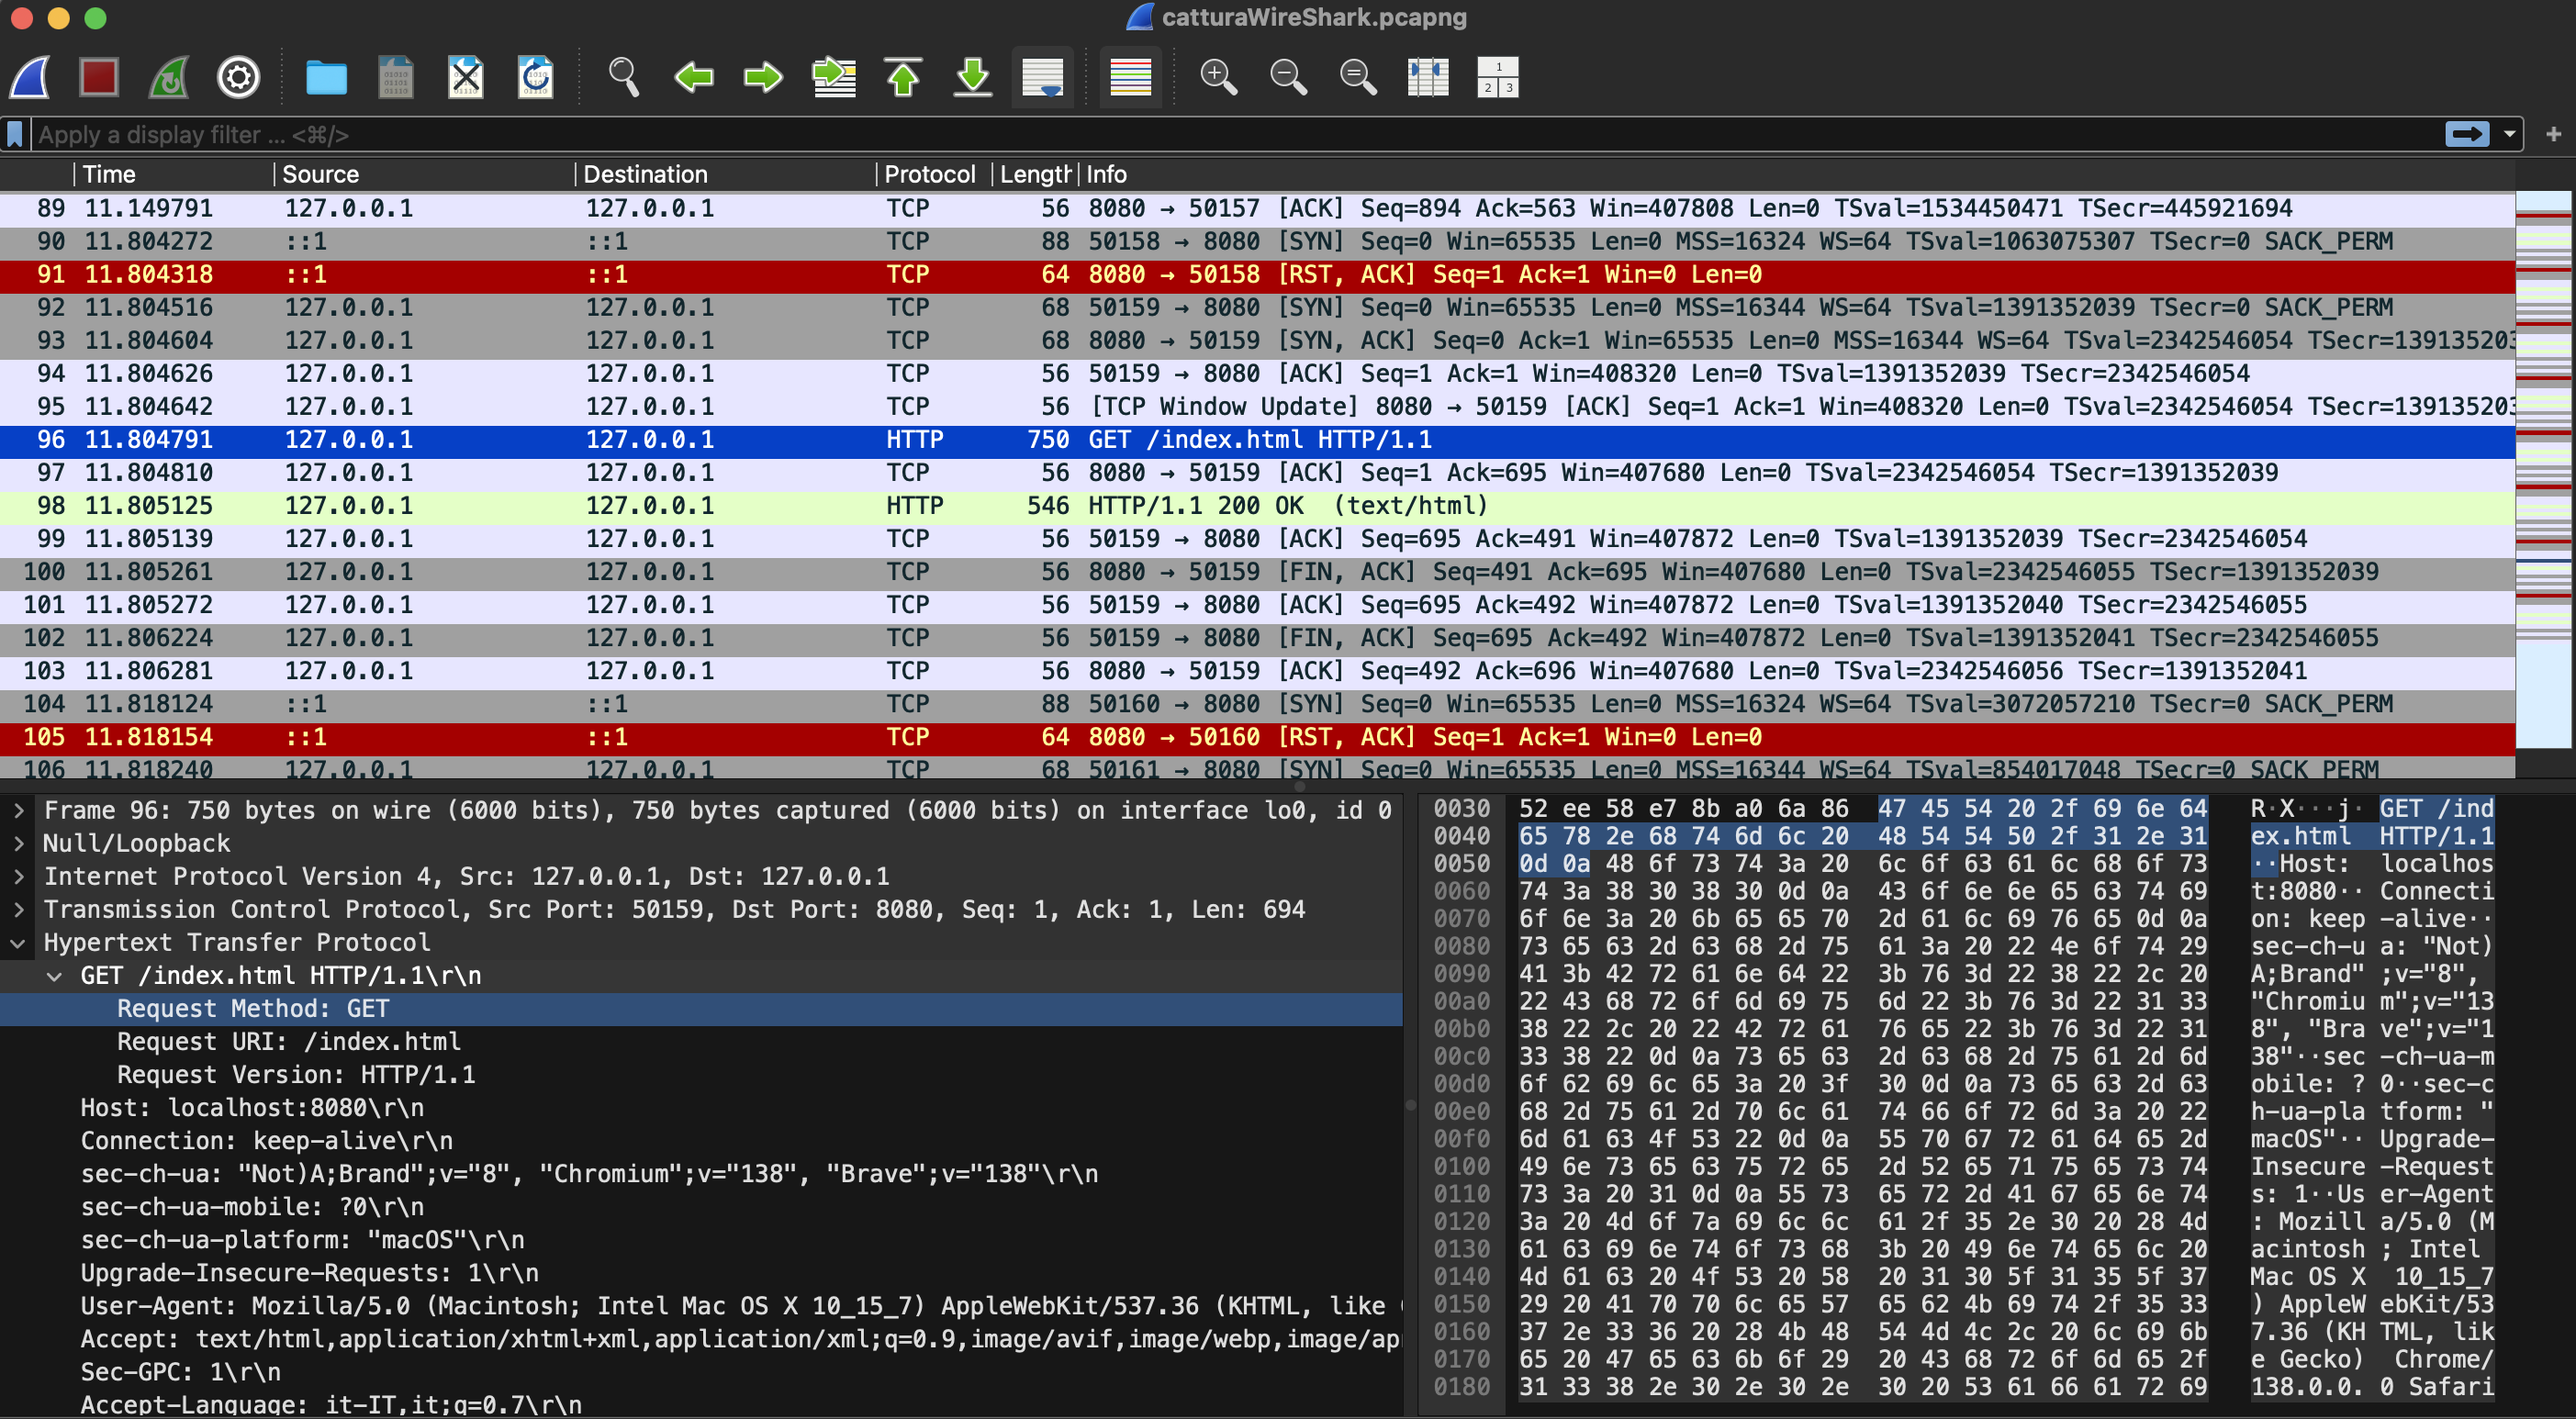
\includegraphics[width=0.9\textwidth]{Images/getRequest.png}
    \caption{Pacchetto HTTP contenente richiesta \texttt{GET}}
\end{figure}

Come si nota dalla sezione “Hypertext Transfer Protocol” di Wireshark, la richiesta include:
\begin{itemize}
    \item Il metodo \texttt{GET}
    \item La versione HTTP \texttt{HTTP/1.1}
    \item Header come \texttt{Host}, \texttt{User-Agent}, ecc.
\end{itemize}

\section{Risposta HTTP con codice \texttt{200 OK}}

A seguito della richiesta, il server restituisce il file richiesto con codice di stato \texttt{200 OK}:

\begin{figure}[H]
    \centering
    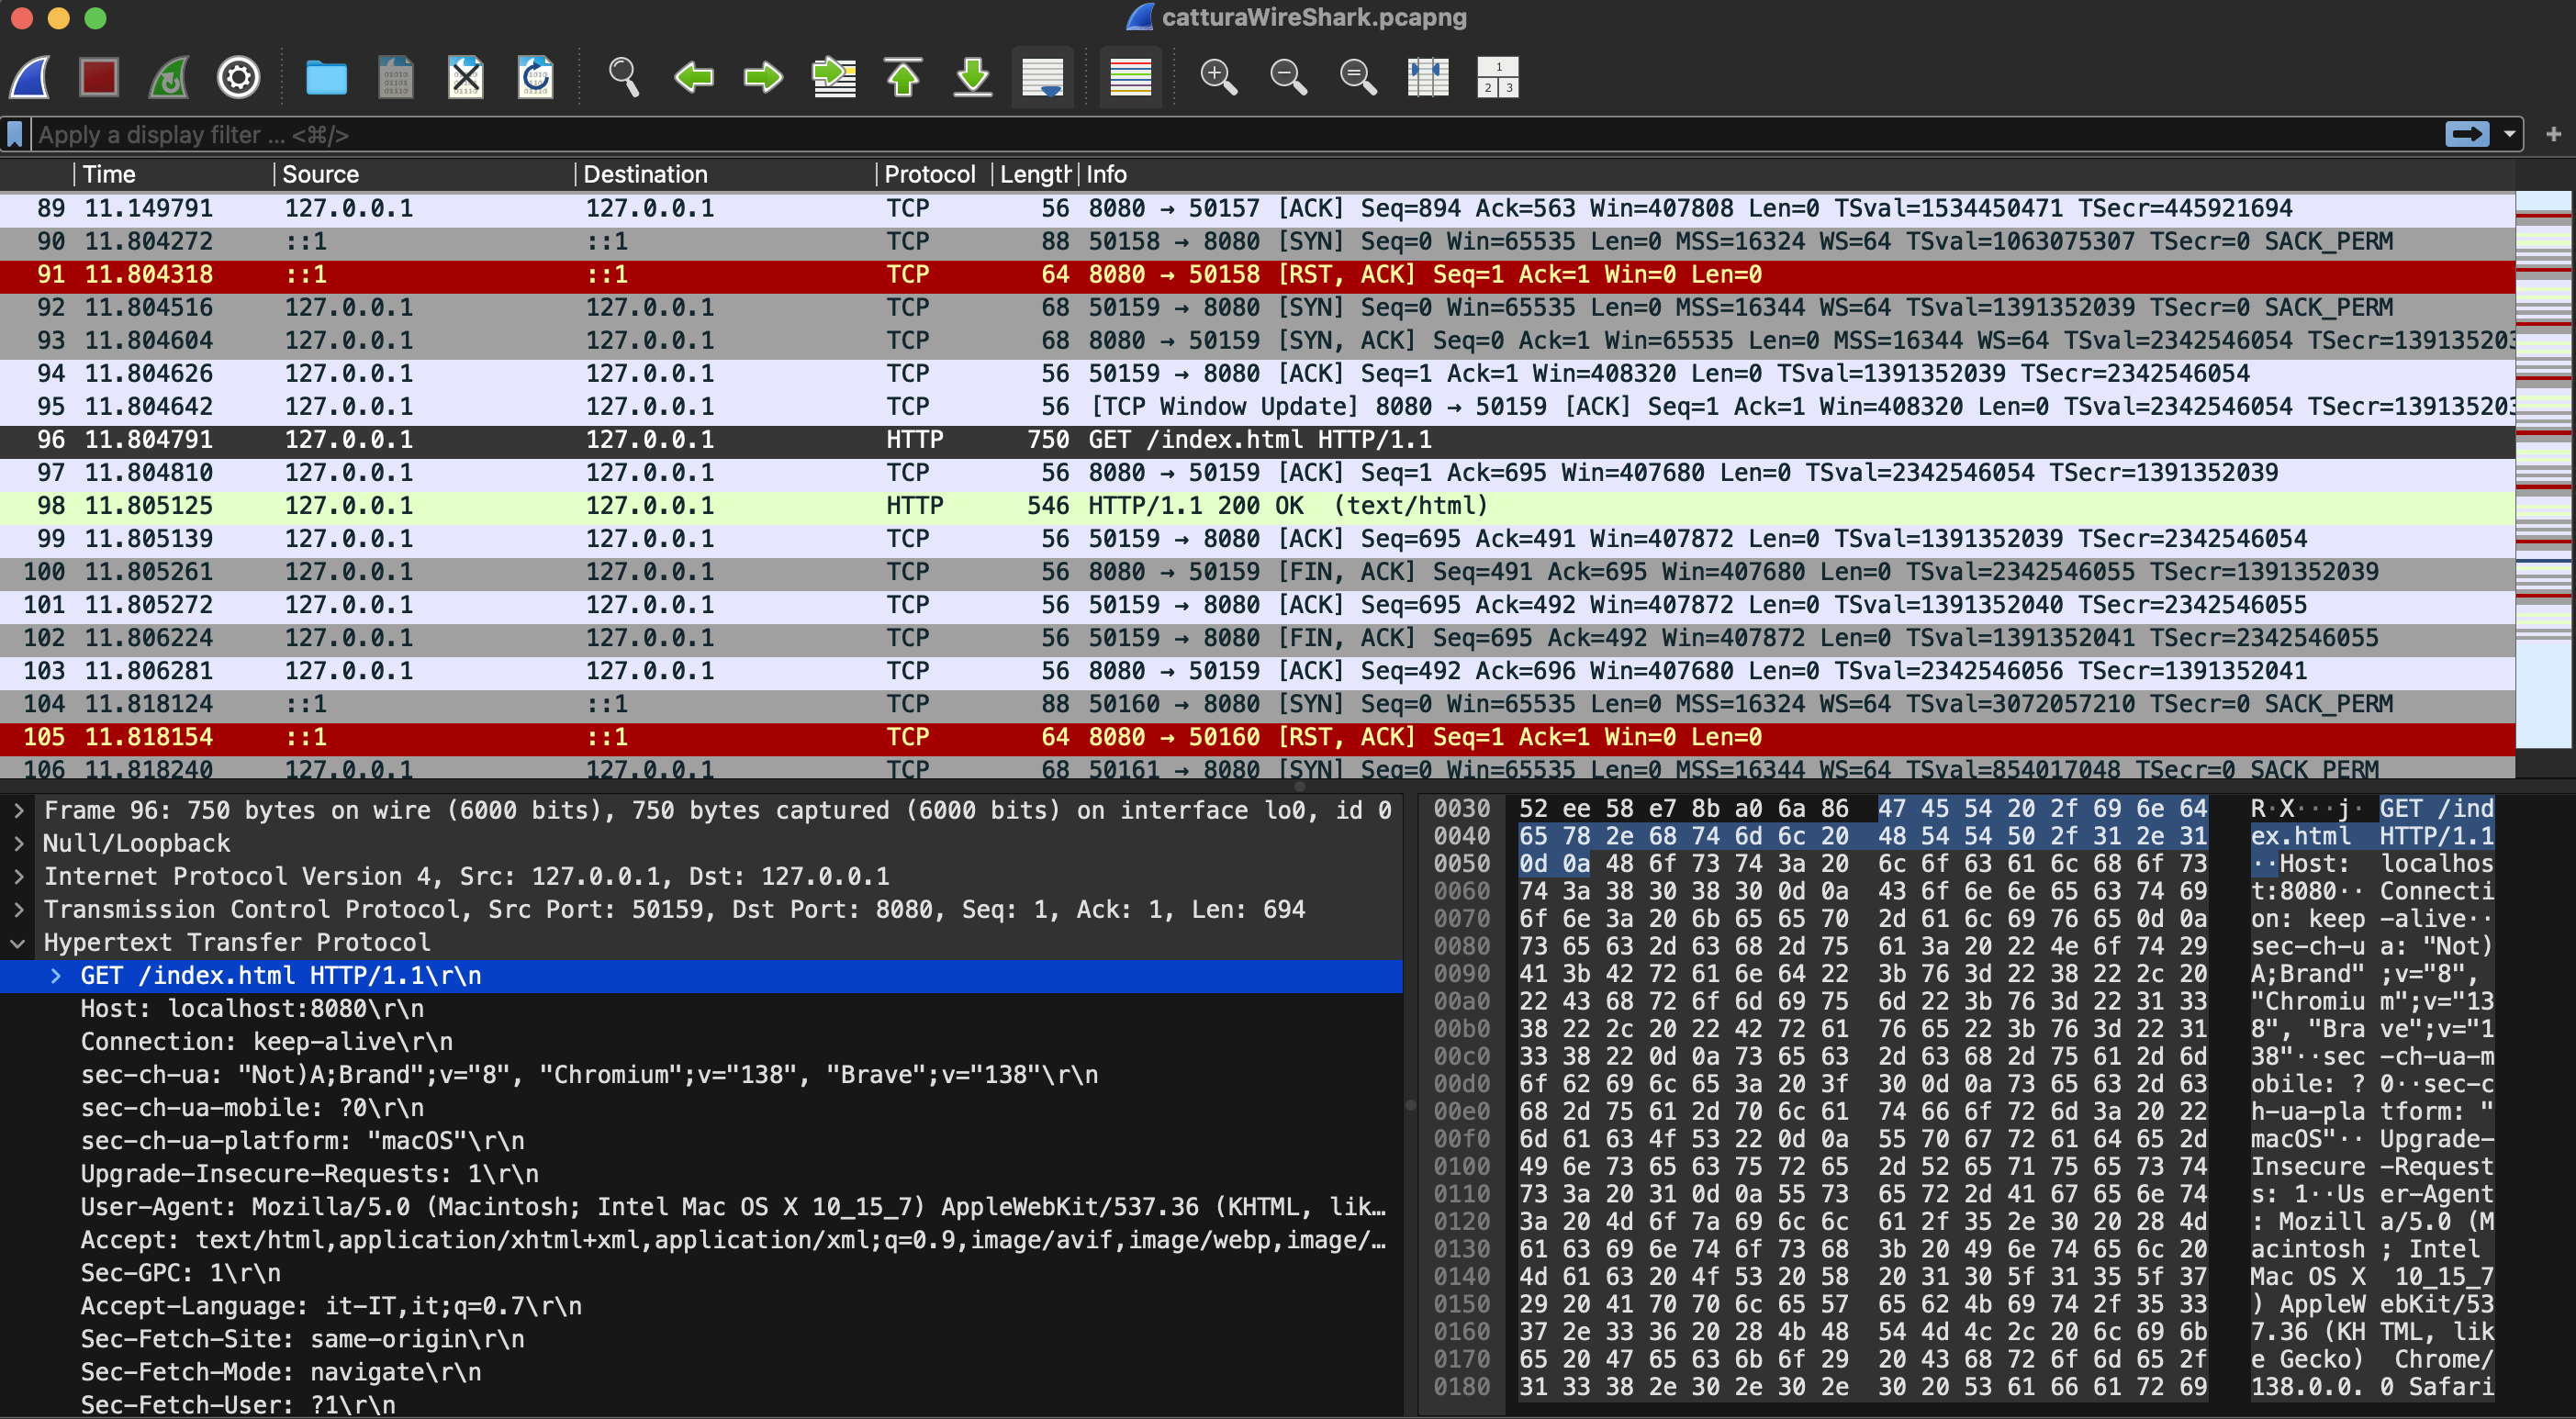
\includegraphics[width=1.0\textwidth]{Images/200.png}
    \caption{Risposta HTTP con codice \texttt{200 OK} e intestazioni corrette}
\end{figure}

L’header della risposta include:
\begin{itemize}
    \item Codice di stato: \texttt{HTTP/1.1 200 OK}
    \item \texttt{Content-Type: text/html}
    \item \texttt{Content-Length}
    \item \texttt{Connection: close}
\end{itemize}

\section{Richiesta di file inesistente: errore \texttt{404}}

Se il client tenta di accedere a una risorsa non esistente (es. \texttt{/contct.html}), il server risponde con il messaggio di errore \texttt{404 Not Found}, come mostrato nella figura seguente:

\begin{figure}[H]
    \centering
    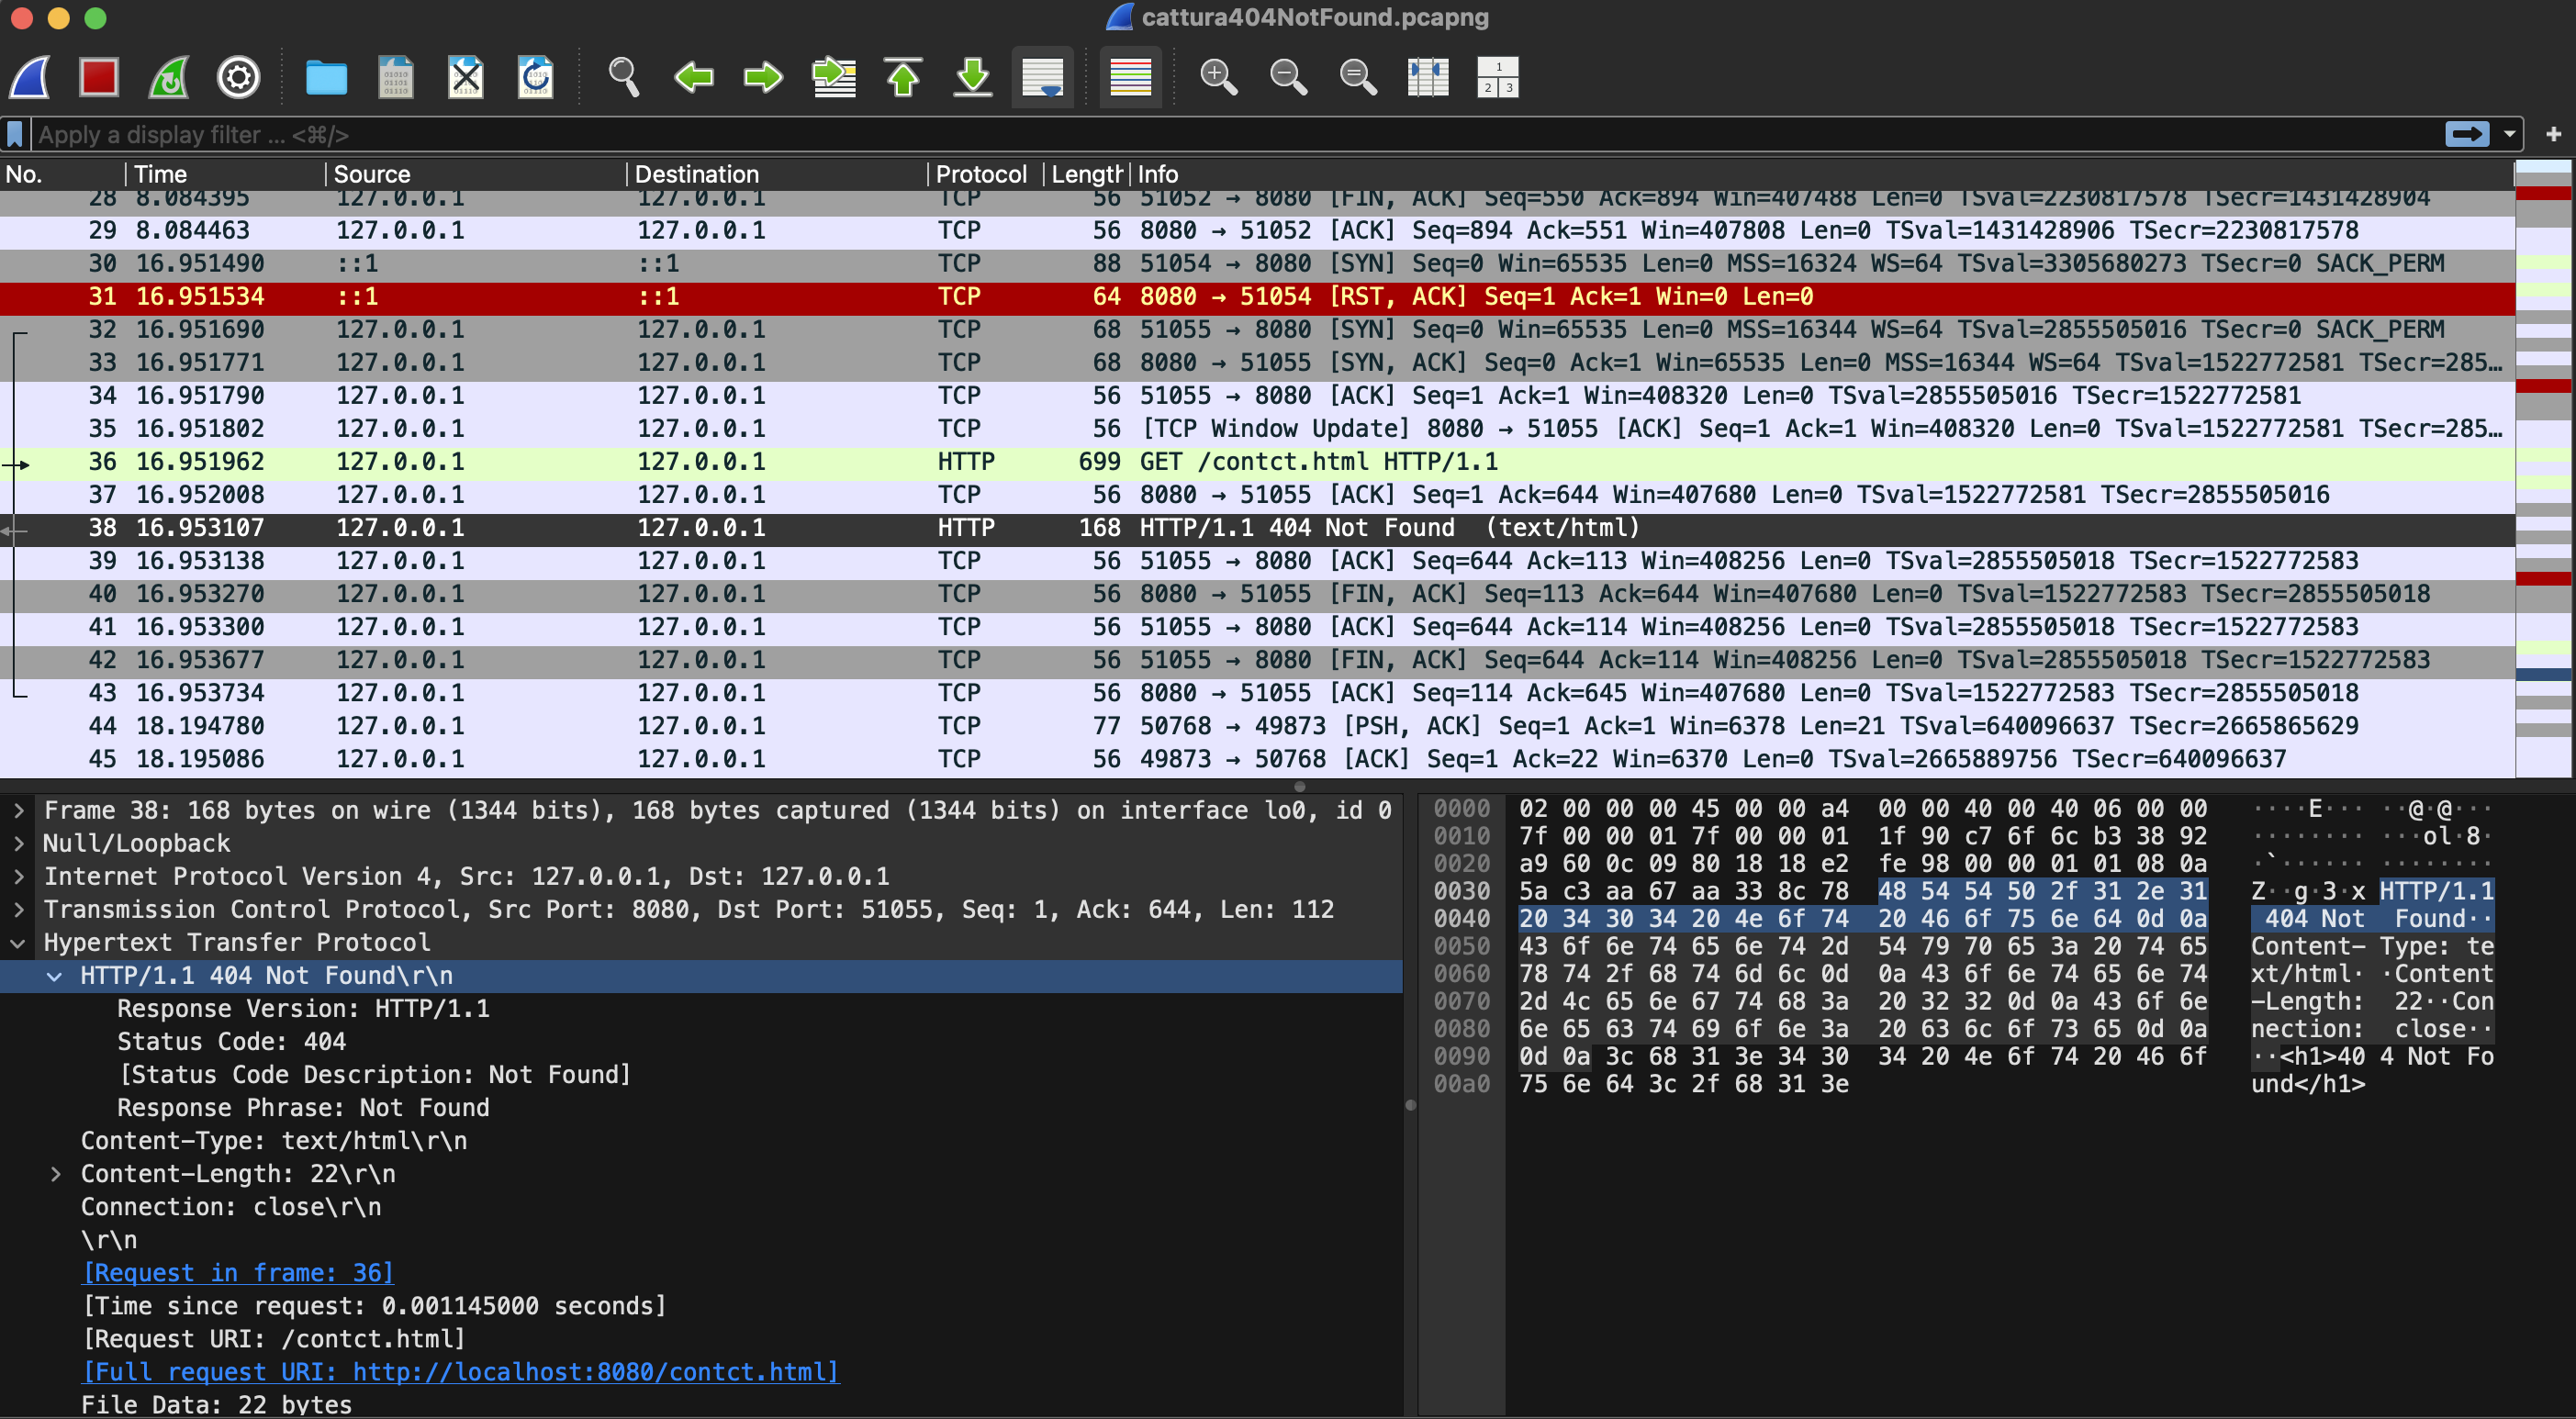
\includegraphics[width=1.0\textwidth]{Images/404NotFound.png}
    \caption{Risposta HTTP con errore \texttt{404 Not Found}}
\end{figure}

\section{Log della console del server}

Per ogni richiesta ricevuta, il server produce un log in console con informazioni utili per il debugging. Un esempio di output è:
\begin{figure}[H]
    \centering
    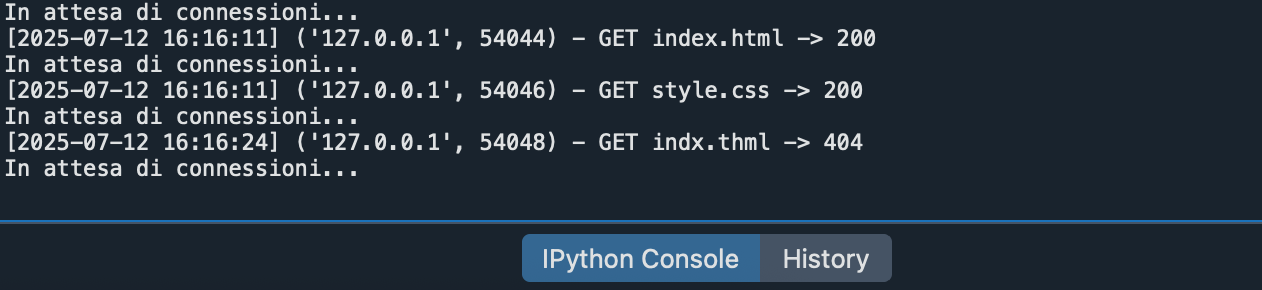
\includegraphics[width=1.0\textwidth]{Images/consoleLog.png}
    \caption{Risposta HTTP con codice \texttt{200 OK} e intestazioni corrette}
\end{figure}

Questo log mostra:
\begin{itemize}
    \item Timestamp della richiesta
    \item Indirizzo IP e porta del client
    \item Metodo e risorsa richiesta
    \item Codice di stato HTTP restituito
\end{itemize}

\chapter{Considerazioni finali }

L’analisi con Wireshark ha confermato che il server genera messaggi HTTP validi secondo specifica e risponde coerentemente a tutte le 
richieste. L’output in console permette di tracciare l’attività del server, facilitando il debugging e l’eventuale estensione futura del
progetto. 
Il server implementa le funzionalità minime di un server HTTP per contenuti statici ma ha molte potenzialità di sviluppo con altre funzionalità,
ad esempio, l'aggiunta di altre pagine, il miglioramento della grafica del sito e del contenuto. 

\end{document}